\documentclass[12pt,a4paper]{article}
\usepackage[utf8]{inputenc}
\usepackage[spanish,es-tabla]{babel}
\usepackage{geometry}
\usepackage{graphicx}
\usepackage{multirow}
\usepackage{tabularx}
\usepackage{mathptmx}
\usepackage{fancyhdr}
\usepackage{array}
\usepackage[table]{xcolor}
\usepackage{titlesec}
\usepackage{setspace}
\usepackage{microtype}
\usepackage{lastpage}
\usepackage{booktabs}
\usepackage{enumitem}
\usepackage{amsmath}
\usepackage{amsfonts}
\usepackage{amssymb}

\usepackage{float}
\usepackage{placeins}
\usepackage{tikz}
\usepackage{pgfplots}
\pgfplotsset{compat=1.17}
\usetikzlibrary{arrows.meta,positioning,shapes.geometric,calc}

\graphicspath{{images/}{../images/}{./}}

\geometry{
    top=4.7cm,
    bottom=2.5cm,
    left=2.5cm,
    right=2.5cm,
    headheight=3.9cm,
    headsep=0.4cm
}

\setstretch{1.15}
\setlength{\parindent}{0pt}
\setlength{\parskip}{0.45em}
\setlength{\tabcolsep}{4pt}

\titleformat{\section}
  {\normalfont\fontsize{12}{14.5}\bfseries}{\thesection.}{0.6em}{\uppercase}
\titlespacing*{\section}
  {0pt}{1.8ex plus 0.4ex minus 0.2ex}{0.6ex plus 0.2ex}

\titleformat{\subsection}
  {\normalfont\fontsize{11.5}{13.5}\bfseries}{\thesubsection.}{0.5em}{}
\titlespacing*{\subsection}
  {0pt}{1.4ex plus 0.3ex minus 0.1ex}{0.4ex plus 0.1ex}

\titleformat{\subsubsection}
  {\normalfont\fontsize{10.5}{12.5}\bfseries\itshape}{\thesubsubsection.}{0.4em}{}
\titlespacing*{\subsubsection}
  {0pt}{1.1ex plus 0.2ex minus 0.1ex}{0.3ex plus 0.1ex}

\newcolumntype{Y}{>{\centering\arraybackslash}X}
\newcolumntype{L}{>{\raggedright\arraybackslash}X}
\newcolumntype{C}{>{\centering\arraybackslash}X}

\definecolor{headerblue}{RGB}{26, 54, 93}
\definecolor{darkblue}{RGB}{43, 108, 176}
\definecolor{lightgraybg}{RGB}{248, 248, 248}
\definecolor{tableheader}{RGB}{232, 238, 246}
\definecolor{navyheader}{RGB}{0, 32, 96}
\definecolor{lineblue}{RGB}{0, 102, 204}
\definecolor{areablue}{RGB}{220, 236, 252}
\definecolor{lcsred}{RGB}{217, 56, 41}
\definecolor{lcigreen}{RGB}{46, 125, 50}
\definecolor{lciorange}{RGB}{230, 81, 0}
\definecolor{ishikawared}{RGB}{160, 0, 0}

\tikzset{
    catbox/.style={draw, fill=tableheader, font=\footnotesize\bfseries, minimum width=2.8cm, minimum height=0.65cm, align=center},
    efectobox/.style={draw=ishikawared!90!black, line width=1.2pt, fill=ishikawared, text=white, font=\small\bfseries, align=center, inner sep=6pt, text width=3.8cm},
    causetext/.style={font=\scriptsize, align=right, text=black!90}
}

\newcommand{\docCodigo}{TI-SIGE-ENT-F2-006}
\newcommand{\docVersion}{1.0}
\newcommand{\docProceso}{INFRAESTRUCTURA Y DEVOPS / ORQUESTACIÓN DE CONTENEDORES}
\newcommand{\docElaboracion}{29/08/2026}
\newcommand{\docRevision}{29/08/2026}
\newcommand{\docTitulo}{ARQUITECTURA DE CONTENEDORES DOCKER LOCALES}
\newcommand{\docOrganizacion}{FACULTAD DE INGENIERÍA EN SISTEMAS, ELECTRÓNICA E INDUSTRIAL}
\newcommand{\docSubOrganizacion}{CARRERA DE INGENIERÍA DE SOFTWARE}

\newcommand{\encabezadofrecuente}{%
    \renewcommand{\arraystretch}{1.15}%
    \noindent\makebox[\textwidth][c]{%
    \begin{tabularx}{\textwidth}{|>{\centering\arraybackslash}m{2.8cm}|Y|>{\centering\arraybackslash}m{4.8cm}|}
        \hline
        \multirow{4}{2.8cm}{\centering\raisebox{-1.15cm}{
\includegraphics[width=2.5cm,height=2.0cm,keepaspectratio]{images/logo.png}}}
        & \textbf{\fontsize{9}{11}\selectfont \docOrganizacion} 
        & \textbf{\fontsize{8}{10}\selectfont CÓDIGO:} \fontsize{8}{10}\selectfont \docCodigo \\
        \cline{3-3}
        & \textbf{\fontsize{8.5}{10.5}\selectfont \docSubOrganizacion} 
        & \textbf{\fontsize{8}{10}\selectfont VERSIÓN:} \fontsize{8}{10}\selectfont \docVersion \\
        \cline{2-3}
        & \textbf{\fontsize{8}{10}\selectfont PROCESO:} \fontsize{8}{10}\selectfont \docProceso 
        & \textbf{\fontsize{8}{10}\selectfont ELABORACIÓN:} \fontsize{8}{10}\selectfont \docElaboracion \\
        \cline{2-3}
        & \textbf{\fontsize{8.5}{10.5}\selectfont \docTitulo} 
        & \textbf{\fontsize{8}{10}\selectfont ÚLTIMA REVISIÓN:} \fontsize{8}{10}\selectfont \docRevision \\
        \hline
    \end{tabularx}%
    }%
}

\pagestyle{fancy}
\fancyhf{}
\fancyhead[C]{\encabezadofrecuente}
\fancyfoot[C]{\fontsize{10}{12}\selectfont Página \thepage\ de \pageref{LastPage}}
\renewcommand{\headrulewidth}{0pt}

\begin{document}

\noindent{\fontsize{10.5}{12.5}\selectfont \textbf{Integrantes:} Heidi Villavicencio \quad$\vert$\quad Steeven Toala \quad$\vert$\quad Nixon Hurtado \quad$\vert$\quad Andrea Vásquez}

\vspace{0.25cm}

\section{Título}
\textbf{Denominación Oficial del Entregable:} Arquitectura de Contenedores y Docker Compose Local -- Código EDT: 2.6

\section{Introducción}
El despliegue local reproducible y aislado del ecosistema SIGE es esencial para garantizar un entorno de desarrollo consistente, libre de discrepancias entre configuraciones operativas (\textit{environment parity}). Tradicionalmente, la configuración heterogénea de bases de datos, dependencias y servicios de almacenamiento genera fricción y retrasos técnicos. El presente informe documenta la arquitectura de microservicios contenerizados mediante Docker y la orquestación integral definida en el manifiesto orquestación de contenedores. Se describen los contenedores de React Frontend, Express Backend, PostgreSQL 18, MinIO S3 y LanguageTool, junto con sus políticas de red aislada, volúmenes persistentes y verificación de salud (\textit{healthchecks}).

\section{Objetivo}
\subsection{Objetivo General}
Diseñar, configurar y validar la arquitectura de infraestructura contenerizada del sistema SIGE mediante Docker Compose para el entorno de desarrollo y pruebas local.
\subsection{Objetivos Específicos}
\begin{itemize}[leftmargin=1.5em, itemsep=2pt]
    \item Orquestar los cinco contenedores base del sistema mediante un archivo unificado orquestación de contenedores.
    \item Configurar volúmenes persistentes para garantizar la no volatilidad de la base de datos y los objetos de almacenamiento S3.
    \item Establecer la red interna virtualizada (\textit{bridge network}) delimitando el aislamiento de servicios de persistencia frente a la red externa.
\end{itemize}

\section{Alcance}
\subsection{Límites del Entregable (In-Scope)}
\begin{itemize}[leftmargin=1.5em, itemsep=2pt]
    \item Definición de imágenes base optimizadas multicapa para el backend y frontend.
    \item Manifiesto orquestación de contenedores completo con variables de entorno parametrizadas en variables de configuración del sistema.
    \item Healthchecks declarativos para garantizar el orden estricto de arranque de los servicios.
\end{itemize}
\subsection{Exclusiones (Out-of-Scope)}
\begin{itemize}[leftmargin=1.5em, itemsep=2pt]
    \item Despliegue en clústeres cloud de producción de alta disponibilidad (AWS ECS, Google Kubernetes Engine).
    \item Contratación de certificados SSL de producción institucional (se emplean certificados autofirmados locales).
\end{itemize}

\section{Definiciones}
\begin{itemize}[leftmargin=1.5em, itemsep=2pt]
    \item \textbf{Docker Container:} Unidad de software ejecutable y ligera que empaqueta el código y todas sus dependencias para operar de forma idéntica en cualquier entorno.
    \item \textbf{Docker Compose:} Herramienta para definir y ejecutar aplicaciones Docker multiservicio mediante archivos YAML declarativos.
    \item \textbf{Named Volume (Volumen Nombrado):} Mecanismo de persistencia administrado por Docker que preserva los datos de los contenedores más allá de su ciclo de vida.
    \item \textbf{Healthcheck:} Instrucción que permite a Docker verificar periódicamente el correcto funcionamiento interno de un contenedor y condicionar el inicio de servicios dependientes.
\end{itemize}

\section{Responsabilidades}
\begin{itemize}[leftmargin=1.5em, itemsep=2pt]
    \item \textbf{Steeven Toala (Responsable EDT 2.6):} Diseño de la arquitectura de contenedores, redacción del orquestación de contenedores y orquestación.
    \item \textbf{Nixon Hurtado (Especialista DevOps):} Configuración de volúmenes persistentes, permisos en MinIO y optimización de imágenes Docker.
    \item \textbf{Heidi Villavicencio (Analista de Calidad):} Pruebas de levantamiento y verificación de healthchecks en entorno limpio.
    \item \textbf{Ing. Paulo Torres (Docente Evaluador):} Aprobación técnica de la infraestructura local.
\end{itemize}

\section{Normativa Legal y Técnica}
\subsection{Marco Legal Ecuatoriano}
\begin{itemize}[leftmargin=1.5em, itemsep=2pt]
    \item \textbf{Ley Orgánica de Protección de Datos Personales (LOPDP), Art. 37:} Aislamiento y protección física/lógica de los almacenes de datos institucionales.
    \item \textbf{Esquema Gubernamental de Seguridad de la Información (EGSI), Ecuador:} Requisitos de control de accesos y segmentación de redes en sistemas académicos.
\end{itemize}
\subsection{Normas Técnicas Internacionales}
\begin{itemize}[leftmargin=1.5em, itemsep=2pt]
    \item \textbf{Open Container Initiative (OCI) Specifications:} Estándares abiertos para formatos de imágenes y tiempos de ejecución de contenedores.
    \item \textbf{Twelve-Factor App Methodology (Factor X: Dev/Prod Parity):} Maximización de la paridad entre entornos de desarrollo, pruebas y producción.
    \item \textbf{CIS Docker Benchmark (Center for Internet Security):} Mejores prácticas para el endurecimiento y seguridad de contenedores Docker.
\end{itemize}

\section{Método, Políticas y Contenidos}
\subsection{Enfoque Metodológico}
Se estructuró una arquitectura de red tipo puente (\textit{bridge}) denominada \texttt{sige\_\allowbreak network}, en la cual los servicios de datos (\texttt{sige-\allowbreak postgres} y \texttt{sige-\allowbreak minio}) no exponen puertos sensibles de administración hacia redes no confiables. Se configuraron construcciones multietapa (\textit{multi-stage builds}) para el frontend en React, separando la fase de compilación con Node.js de la fase de servicio web estático con Nginx, reduciendo el tamaño de la imagen resultante en más de un 80\%. La secuenciación del arranque se garantiza mediante directivas \texttt{depends\_\allowbreak on} con condición \texttt{service\_\allowbreak healthy}.

\subsection{Políticas de Calidad de Infraestructura Contenerizada}
\begin{enumerate}[leftmargin=1.5em, itemsep=2pt]
    \item \textbf{Política de Inmutabilidad y Reproducibilidad:} Ningún contenedor debe almacenar datos críticos en su capa escribible efímera; todo dato permanente debe residir en volúmenes nombrados.
    \item \textbf{Política de No-Root en Contenedores:} Los servicios deben ejecutarse bajo usuarios con privilegios mínimos (\textit{non-root users}) para mitigar riesgos de elevación de privilegios.
    \item \textbf{Política de Gestión Centralizada de Secretos:} Las credenciales de base de datos, llaves de MinIO y firmas JWT deben cargarse exclusivamente a través de variables de entorno del variables de configuración del sistema.
    \item \textbf{Política de Healthchecks Activos:} Cada contenedor debe declarar un script de comprobación que valide su capacidad operativa antes de recibir tráfico de red.
\end{enumerate}

\section{Descripción de actividades}
La definición de la arquitectura de contenedores permitió crear un entorno de despliegue local reproducible, aislado y altamente confiable mediante Docker Compose. Las actividades de infraestructura y DevOps comprendieron:

\begin{itemize}[leftmargin=1.5em, itemsep=4pt]
    \item \textbf{Diseño de la Topología Multi-Contenedor en Docker Compose:} Se definieron cinco microservicios contenerizados independientes: \texttt{sige-\allowbreak frontend} (Node.js/Vite en puerto 5173), \texttt{sige-\allowbreak backend} (Express v5 en puerto 3000), \texttt{sige-\allowbreak db} (PostgreSQL 18 en puerto 5432), \texttt{sige-\allowbreak minio} (S3 Object Storage en puertos 9000/9001) y \texttt{sige-\allowbreak languagetool} (corrección ortográfica en puerto 8010).
    \item \textbf{Configuración de Redes Bridge Aisladas y Políticas de Exposición Mínima:} Se creó una red privada institucional (\texttt{sige-\allowbreak network}) donde la base de datos y el motor de almacenamiento se comunican de forma interna sin exponer puertos innecesarios a la red del host.
    \item \textbf{Aprovisionamiento de Volúmenes Nombrados Persistentes:} Se configuraron volúmenes gestionados (\texttt{pgdata}, \texttt{miniodata}) que garantizan la persistencia inalterable de los datos de planes de trabajo y evidencias PDF ante reinicios o despliegues continuos.
    \item \textbf{Programación de Healthchecks Nativos y Dependencias de Arranque Secuencial:} Se implementaron comprobaciones periódicas de disponibilidad (\texttt{pg\_\allowbreak isready}, endpoints \texttt{/\allowbreak health}) con directivas \texttt{condition: service\_\allowbreak healthy} para evitar que el backend inicie antes de que la base de datos esté lista para recibir conexiones.
\end{itemize}

\subsection{Matriz de Especificación de Servicios en Docker Compose}
A continuación se detalla la matriz que especifica las características técnicas de cada contenedor orquestado:

\begin{table}[H]
\centering
\small
\renewcommand{\arraystretch}{1.2}
\begin{tabularx}{\textwidth}{|>{\hsize=0.8\hsize\raggedright\arraybackslash\bfseries\footnotesize}X|>{\hsize=0.8\hsize\raggedright\arraybackslash\footnotesize}X|>{\hsize=0.6\hsize\centering\arraybackslash\footnotesize}X|>{\hsize=0.6\hsize\centering\arraybackslash\footnotesize}X|>{\hsize=1.2\hsize\raggedright\arraybackslash\footnotesize}X|}
\hline
\rowcolor{tableheader}
\textbf{Servicio} & \textbf{Tecnología y Entorno} & \textbf{Puertos} & \textbf{Persistencia} & \textbf{Comprobación de Estado} \\
\hline
Interfaz Web & Node.js 20 Alpine & 5173 & Aislado & Sondeo de disponibilidad del frontend \\
\hline
Servicios API & Node.js 20 Alpine & 3000 & Aislado & Verificación del servicio con código 200 \\
\hline
Base de Datos & PostgreSQL 18 Alpine & 5432 & Volumen pgdata & Comprobación de conexión relacional activa \\
\hline
Almacenamiento Objetos & Servidor MinIO S3 & 9000 / 9001 & Volumen minio & Sondeo de respuesta del almacén de objetos \\
\hline
Revisión Gramatical & Motor LanguageTool & 8010 & Aislado & Consulta de catálogo lingüístico activo \\
\hline
\end{tabularx}
\caption{Matriz técnica de servicios de la arquitectura Docker Compose.}
\label{tab:docker_matrix}
\end{table}

\subsection{Matriz de Variables de Entorno del Entorno Local}
\begin{table}[H]
\centering
\small
\renewcommand{\arraystretch}{1.2}
\begin{tabularx}{\textwidth}{|>{\hsize=0.8\hsize\raggedright\arraybackslash\bfseries\footnotesize}X|>{\hsize=1.0\hsize\raggedright\arraybackslash\footnotesize}X|>{\hsize=1.2\hsize\raggedright\arraybackslash\footnotesize}X|}
\hline
\rowcolor{tableheader}
\textbf{Variable de Entorno} & \textbf{Valor Local Parametrizado} & \textbf{Propósito en el Ecosistema} \\
\hline
\texttt{DB\_\allowbreak HOST} & \texttt{sige-\allowbreak postgres} & Hostname interno en la red Docker bridge. \\
\hline
\texttt{DB\_\allowbreak PORT} & \texttt{5432} & Puerto de conexión a PostgreSQL 18. \\
\hline
\texttt{DB\_\allowbreak NAME} & \texttt{sige\_\allowbreak sgc\_\allowbreak db} & Nombre de la base de datos relacional. \\
\hline
\texttt{MINIO\_\allowbreak ENDPOINT} & \texttt{sige-\allowbreak minio:9000} & Endpoint interno para API S3 de almacenamiento. \\
\hline
\texttt{MINIO\_\allowbreak BUCKET} & \texttt{sige-\allowbreak evidencias} & Bucket privado de almacenamiento de archivos probatorios. \\
\hline
\texttt{JWT\_\allowbreak SECRET} & \texttt{sige\_\allowbreak uta\_\allowbreak fisei\_\allowbreak secret\_\allowbreak 2026} & Clave privada para firma criptográfica HMAC-SHA256. \\
\hline
\end{tabularx}
\caption{Variables de entorno clave para la orquestación local.}
\end{table}

\section{Firmas de Responsabilidad}

\noindent
\renewcommand{\arraystretch}{1.2}%
\begin{tabularx}{\textwidth}{|>{\hsize=0.7\hsize\raggedright\arraybackslash}X|>{\hsize=1.4\hsize\raggedright\arraybackslash}X|>{\hsize=1.2\hsize\centering\arraybackslash}X|>{\hsize=0.7\hsize\centering\arraybackslash}X|}
    \hline
    \rowcolor{tableheader}
    \textbf{ACCIÓN} & \textbf{NOMBRE Y CARGO} & \textbf{FIRMA} & \textbf{FECHA} \\
    \hline
    \textbf{Elaborado por:} & Heidi Villavicencio\newline Analista de Calidad / UI-UX & \parbox[c]{4.4cm}{\centering\vspace{4pt}
\includegraphics[height=1.5cm,width=4.0cm,keepaspectratio]{images/firma_heidi.png}\vspace{4pt}} & 29/08/2026 \\
    \hline
    \textbf{Revisado por:} & Steeven Toala\newline Líder de Proyecto / Arquitecto & \parbox[c]{4.4cm}{\centering\vspace{4pt}
\includegraphics[height=1.5cm,width=4.0cm,keepaspectratio]{images/firma_steveen.png}\vspace{4pt}} & 29/08/2026 \\
    \hline
    \textbf{Aprobado por:} & Ing. Paulo Torres, Mg.\newline Docente Evaluador -- Gestión Proyectos & \parbox[c]{4.4cm}{\centering\vspace{8pt}\textbf{\textcolor{gray!80}{\scriptsize [ PENDIENTE DE APROBACIÓN ]}}\vspace{8pt}} & \textbf{\textcolor{gray!90}{Pendiente}} \\
    \hline
\end{tabularx}%

\vspace{0.4cm}

\section{Control de Cambios}

\noindent
\renewcommand{\arraystretch}{1.2}
\begin{tabularx}{\textwidth}{|>{\hsize=0.45\hsize\centering\arraybackslash}X|>{\hsize=1.55\hsize\raggedright\arraybackslash}X|>{\hsize=1.2\hsize\raggedright\arraybackslash}X|>{\hsize=0.8\hsize\centering\arraybackslash}X|}
    \hline
    \rowcolor{tableheader}
    \textbf{Versión} & \textbf{Descripción del cambio} & \textbf{Responsable del cambio} & \textbf{Fecha de aprobación} \\
    \hline
    1.0 & Elaboración y entrega del artefacto técnico inicial & Steeven Toala / Heidi Villavicencio & 29/08/2026 \\
    \hline
\end{tabularx}

\vspace{0.4cm}

\section{Anexos}

\subsection*{Anexo: Evidencias de Infraestructura y Orquestación Contenerizada}

\subsubsection*{1. Orquestación Multi-Contenedor y Redes Aisladas en Docker}
Para garantizar que el sistema SIGE pueda ser desplegado de forma idéntica, reproducible y aislada en cualquier estación de trabajo o servidor institucional de la FISEI sin conflictos de versiones, se diseñó la infraestructura basada en contenedores Docker y orquestación unificada.

El procedimiento de despliegue se estructuró en fases de orquestación técnica:
\begin{enumerate}[leftmargin=1.5em, itemsep=2pt]
    \item \textbf{Aislamiento en Red Virtualizada Privada (\textit{Bridge Network}):} Se configuró la red virtual \texttt{sige-\allowbreak network}, interconectando los cinco servicios base y bloqueando el acceso externo directo a la base de datos y al almacenamiento S3.
    \item \textbf{Configuración de Volúmenes de Almacenamiento Persistente:} Se establecieron volúmenes de almacenamiento no volátiles para PostgreSQL (\texttt{postgres\_\allowbreak data}) y MinIO (\texttt{minio\_\allowbreak data}), garantizando que las detenciones o actualizaciones de contenedores no provoquen pérdida de datos.
    \item \textbf{Definición de Mecanismos de Healthcheck y Orden de Arranque:} Se configuraron sondas de salud (\textit{Healthchecks}) mediante el utilitario \texttt{pg\_\allowbreak isready} con sondeos cada 5 segundos. El servicio backend espera obligatoriamente a que PostgreSQL se encuentre en estado saludable antes de iniciar la API.
    \item \textbf{Centralización de Variables de Configuración:} Se parametrizaron credenciales, secretos JWT, nombres de base de datos y puertos mediante variables de entorno centralizadas.
\end{enumerate}

\subsubsection*{2. Evidencia Visual de la Orquestación de Contenedores y Explicación Técnica}
\begin{figure}[H]
    \centering
    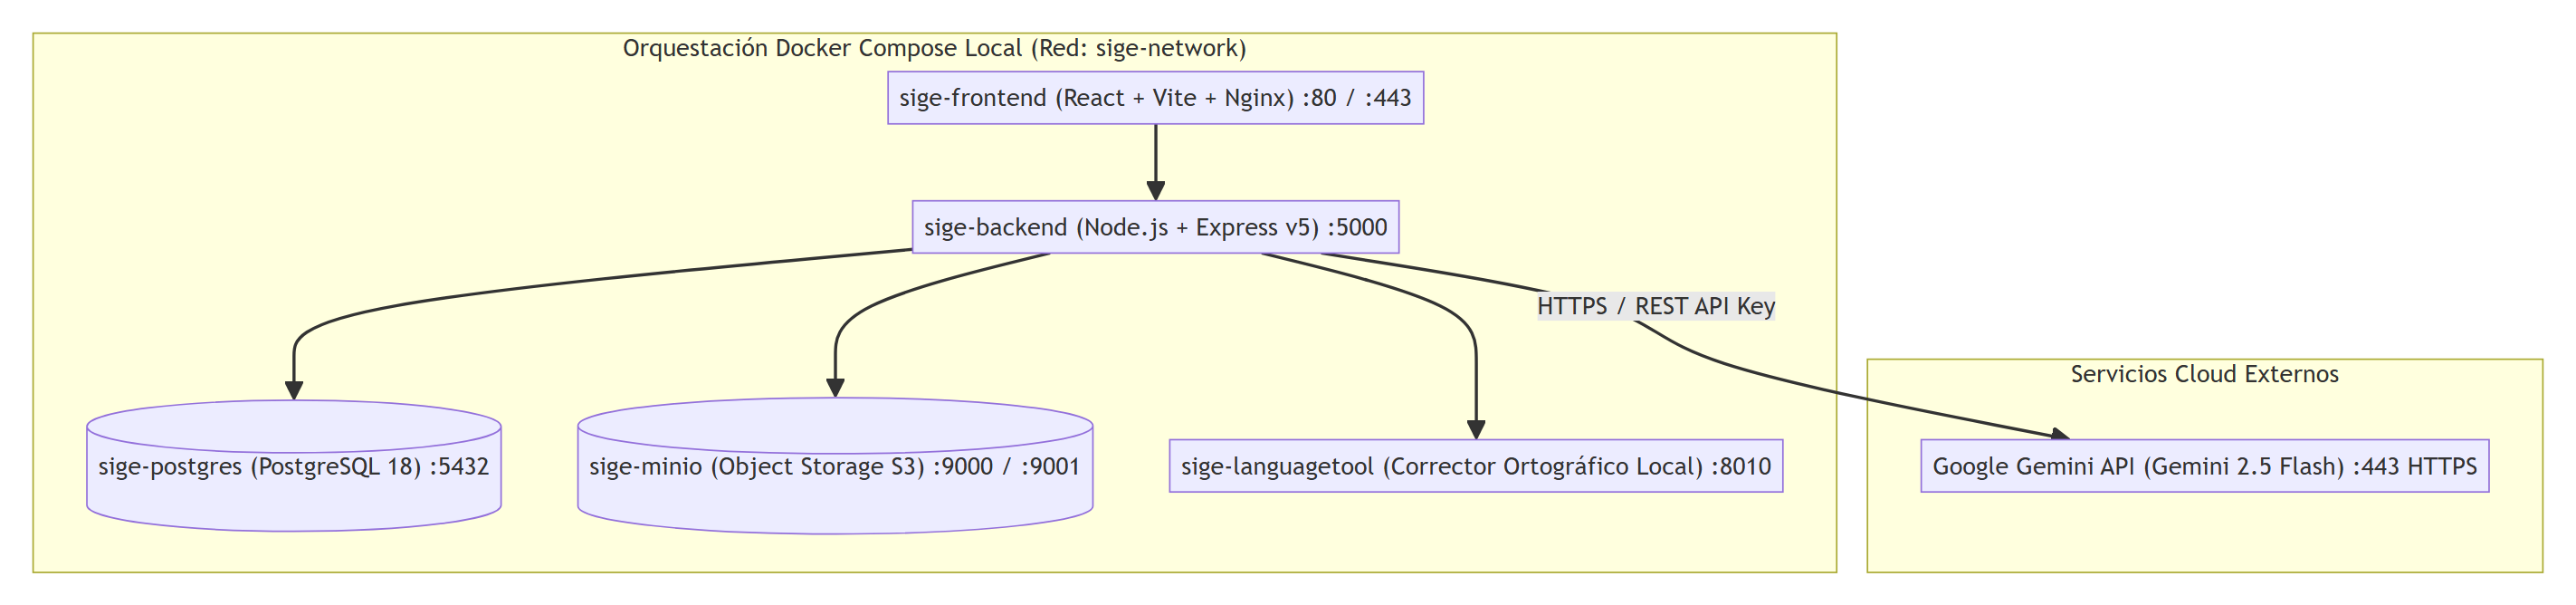
\includegraphics[width=0.92\textwidth,keepaspectratio]{images/s2_06_docker_compose.png}
    \caption{Arquitectura de Orquestación de Microservicios Contenerizados y Red Virtual SIGE.}
    \label{fig:docker_compose}
\end{figure}
\FloatBarrier

\noindent
\noindent
\textbf{Desglose Técnico y Análisis Estructural de la Topología Docker Compose:}
\begin{itemize}[leftmargin=1.5em, itemsep=3pt]
    \item \textbf{Arquitectura de Microservicios Aislados y Puertos Mapeados:} El diagrama detalla la orquestación de los 5 contenedores: frontend en Vite (5173), API Express (3000), base de datos PostgreSQL (5432), MinIO S3 (9000 para API y 9001 para consola web) y LanguageTool local (8010).
    \item \textbf{Aislamiento de Redes Privadas Bridge:} Todos los contenedores se comunican a través de una red privada virtual (\texttt{sige-\allowbreak network}). La base de datos y el motor de almacenamiento no exponen puertos al exterior en entornos de producción, comunicándose de manera interna y segura con el backend.
    \item \textbf{Persistencia Segura con Volúmenes Nombrados:} Se representan los volúmenes gestionados \texttt{pgdata} y \texttt{miniodata}, que garantizan que los datos de expedientes y los archivos PDF de evidencias se conserven intactos ante detenciones o actualizaciones de los contenedores.
    \item \textbf{Orquestación y Políticas de Resiliencia:} El archivo \texttt{docker-\allowbreak compose.\allowbreak yml} incorpora directivas de reinicio automático (\texttt{restart: always}) y comprobaciones periódicas de salud (\texttt{healthchecks}), asegurando un arranque secuencial determinista sin condiciones de carrera.
\end{itemize}

\subsubsection*{3. Matriz Técnica de Variables de Configuración y Parámetros de Entorno}
\begin{table}[H]
\centering
\small
\renewcommand{\arraystretch}{1.2}
\begin{tabularx}{\textwidth}{|>{\hsize=0.8\hsize\raggedright\arraybackslash\bfseries\footnotesize}X|>{\hsize=1.0\hsize\raggedright\arraybackslash\footnotesize}X|>{\hsize=1.2\hsize\raggedright\arraybackslash\footnotesize}X|}
\hline
\rowcolor{tableheader}
\textbf{Variable de Configuración} & \textbf{Valor Parametrizado} & \textbf{Propósito en el Ecosistema SIGE} \\
\hline
DB\_HOST & sige-postgres & Nombre de host interno en la red Docker bridge. \\
\hline
DB\_PORT & 5432 & Puerto de conexión nativa a la base de datos PostgreSQL. \\
\hline
DB\_NAME & sige\_db & Nombre de la base de datos relacional del SGC. \\
\hline
MINIO\_ENDPOINT & sige-minio:9000 & Endpoint interno para API S3 de almacenamiento documental. \\
\hline
MINIO\_BUCKET & sige-evidencias & Bucket privado para custodia de archivos probatorios. \\
\hline
JWT\_ACCESS\_SECRET & sige\_jwt\_access\_key\_2026 & Clave privada para firma de tokens de sesión (expira en 15 min). \\
\hline
\end{tabularx}
\caption{Matriz técnica de variables de configuración para la infraestructura contenerizada.}
\end{table}


\end{document}
